\documentclass{beamer}

\usepackage[utf8]{inputenc}
\usepackage[frenchb]{babel}
\usepackage{verbatim}
\usepackage{graphicx}
\usepackage{color}
\usepackage{hyperref}
\usepackage{verbatim}
\usepackage{url}
\usepackage{auto-pst-pdf}
\usepackage{pst-plot}
\usepackage{moreverb}
\usepackage{fancyvrb}
\usepackage{minted}
\usepackage{algpseudocode}
\usepackage{natbib}
\usepackage{eulervm}

\hypersetup{colorlinks=true, linkcolor=black, urlcolor=blue}
\usetheme{boxes}
\beamertemplatenavigationsymbolsempty
\setbeamertemplate{sections/subsections in toc}[circle]
\setbeamertemplate{footline}[frame number]
\setbeamertemplate{itemize items}[circle]
\setbeamertemplate{itemize subitem}[square]

\title{{\bf Understanding Random Forests}\\
From Theory to Practice}
\author{Gilles Louppe}
\institute{Université de Liège, Belgium}
\date{October 9, 2014}

\newcommand{\todo}[1]{\textcolor{red}{[TODO] #1}}

\definecolor{lightgreen}{rgb}{0.0,0.8,0.0}
\definecolor{lightblue}{rgb}{0.3,0.8,1.0}
\definecolor{lightred}{rgb}{0.874,0.180,0.105}
\definecolor{gray}{rgb}{0.4,0.4,0.4}
\definecolor{lightgray}{rgb}{0.8,0.8,0.8}
\definecolor{shadecolor}{rgb}{0.9,0.9,0.9}
\newrgbcolor{mygreen}{.00 .5 .00}
\newrgbcolor{myyellow}{.6 .6 .00}

\DeclareMathOperator*{\argmax}{arg\,max}


\newrgbcolor{mygreen}{.00 .5 .00}
\newcommand{\X}[1]{\textcolor{blue}{#1}}
\newcommand{\y}[1]{\textcolor{red}{#1}}
\newcommand{\model}[1]{\textcolor{mygreen}{#1}}
\newcommand{\loss}[1]{\textcolor{lightblue}{#1}}

\begin{document}

% Title page ==================================================================

\begin{frame}
\titlepage
\end{frame}


% Motivation ==================================================================

\begin{frame}
  \frametitle{Outline}
  \tableofcontents
\end{frame}

\section{Motivation}
% Mention what is not included in this talk

\begin{frame}{Motivation}

\begin{figure}
\vspace{-0.5cm}
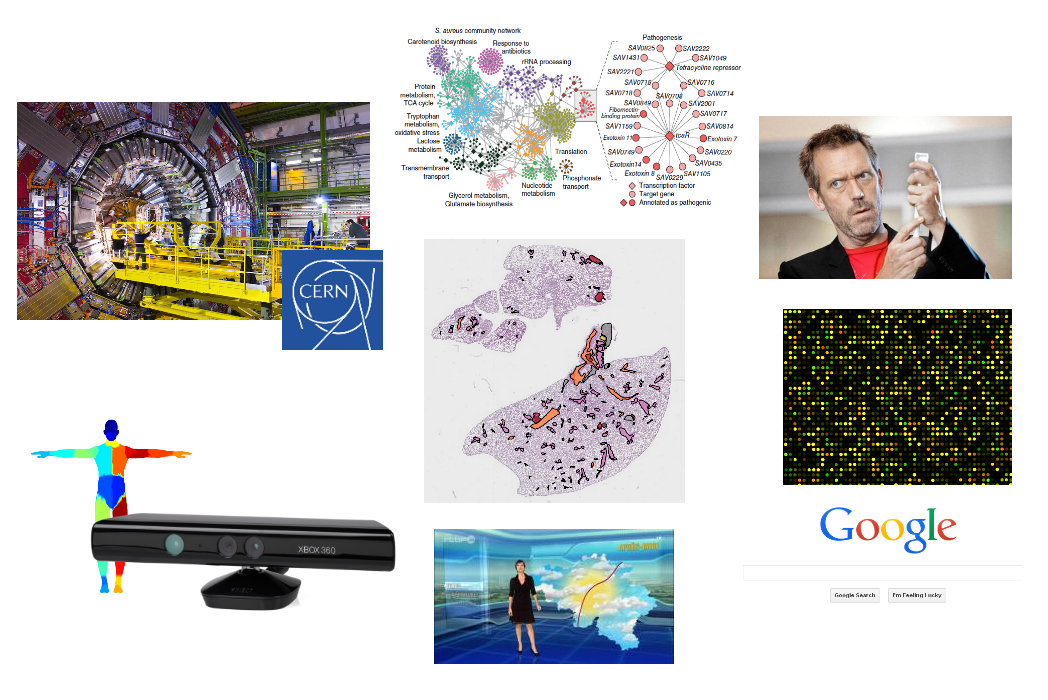
\includegraphics[scale=0.4]{./figures/motivation.png}
\end{figure}

% concrete example => predict output from a set of measurements
% use a continuous example all throughout the slides
% quality of wine from physicochemical properties
\end{frame}

\begin{frame}{Objective}

\begin{center}
From a set of {\bf \X{measurements}},

\vspace{1cm}

learn a {\bf \model{model}}

\vspace{1cm}

to predict and understand {\bf \y{a phenomenon}}.

\end{center}

\end{frame}

\begin{frame}{Running example}

\begin{columns}
\begin{column}{0.5\textwidth}

\begin{center}
From {\bf \X{physicochemical properties}} (alcohol, acidity, sulphates, ...),

\vspace{1cm}

learn a {\bf \model{model}}

\vspace{1cm}

to predict {\bf \y{wine taste preferences}} (from 0 to 10).

\end{center}

\end{column}
\begin{column}{0.5\textwidth}
  \begin{figure}
  \vspace{-0.5cm}
  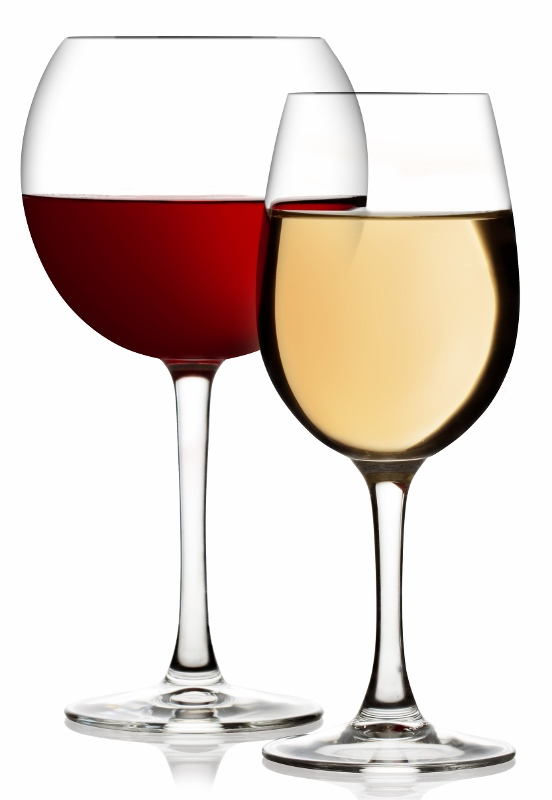
\includegraphics[scale=0.6]{./figures/wine.jpg}
  \end{figure}
\end{column}
\end{columns}

\vspace{1cm}

{\footnotesize
P. Cortez, A. Cerdeira, F. Almeida, T. Matos and J. Reis,
{\it Modeling wine preferences by data mining from physicochemical properties},
2009.}


\end{frame}


% Supervised learning =========================================================

\AtBeginSection[]
{
\begin{frame}
  \frametitle{Outline}
  \tableofcontents[currentsection]
  % Die Option [pausesections]
\end{frame}
}

\section{Growing decision trees}

\begin{frame}{Supervised learning}

\begin{itemize}
\item The inputs are random variables \X{$X = X_1$, ..., $X_p$};
\item The output is a random variable \y{$Y$}.
\end{itemize}

\begin{itemize}
\item Data comes as a finite learning set $${\cal L} = \{(\X{\mathbf{x}_i}, \y{y_i}) | i = 0, \dots, N-1 \},$$
where \X{$\mathbf{x}_i \in {\cal X} = {\cal X}_1 \times ... \times {\cal X}_p$} and \y{$y_i \in {\cal Y}$}
are randomly drawn from $P_{\X{X},\y{Y}}$.
\end{itemize}

\begin{itemize}
\item The goal is to find a model $\model{\varphi_{\cal L}}: \X{{\cal X}} \mapsto \y{{\cal Y}}$ minimizing
$$
Err(\model{\varphi_{\cal L}}) = \mathbb{E}_{\X{X}, \y{Y}}\{ L(\y{Y}, \model{\varphi_{\cal L}}(\X{X})) \}.
$$
\end{itemize}

\end{frame}

\begin{frame}{Performance evaluation}
Depending on the problem, errors are not measured in the same way.

\begin{itemize}

\item {\it Classification} (e.g. ${\cal Y} = \{ \text{yes}, \text{no} \}$):
  $$L(Y, \varphi_{\cal L}(X)) = 1(Y \neq \varphi_{\cal L}(X))$$
  {\it \footnotesize (Number of times the predictions are wrong.)}

\item {\it Regression} (e.g. ${\cal Y} = \mathbb{R}$):
  $$L(Y, \varphi_{\cal L}(X)) = (Y - \varphi_{\cal L}(X))^2$$
  {\it \footnotesize (Large errors are more penalized.)}

\end{itemize}

\end{frame}


% Decision trees ==============================================================

\begin{frame}{Decision trees}
% relate criterion to performance
\end{frame}


% Forests =====================================================================

\begin{frame}{Random forests}
\end{frame}


% Bias-variance ===============================================================

\begin{frame}{Bias-variance trade-off}
% Condorcet Jurys theorem => make people vote on wine quality
% Answer why making several trees help reduce the error
% even if they are built at random!
\end{frame}


% Bias-variance ===============================================================

\section{Interpreting random forests}

\begin{frame}{Reading decision trees}
% Show a tree
% Show a forest! <= limitation + there may be several ways to explain the ouput
\end{frame}

\begin{frame}{Variable importances}
% Show them => How to interpret them?
% MDA + MDI
\end{frame}

\begin{frame}{Mean decrease of impurity}
% Motivation
\end{frame}

\begin{frame}{Working assumptions}
\end{frame}

\begin{frame}{Result 1: Three-level decomposition}
\end{frame}

\begin{frame}{Result 2: Irrelevant variables}
\end{frame}

\begin{frame}{Non-totally randomized trees}
\end{frame}

\begin{frame}{Further insights}
% Source of bias
\end{frame}


% Computational performance ===================================================

\section{Computational performance}

\begin{frame}{Complexity}
\end{frame}

\begin{frame}{Implementation}
\end{frame}

\begin{frame}{Random patches}
\end{frame}


% Conclusions =================================================================

\section{Conclusions}

\begin{frame}{Conclusions}
\end{frame}

\end{document}
